\documentclass[a4paper]{article}
\usepackage[utf8]{inputenc}
\usepackage[spanish, es-tabla, es-noshorthands]{babel}
\usepackage[table,xcdraw]{xcolor}
\usepackage[a4paper, footnotesep = 1cm, width=20cm, top=2.5cm, height=25cm, textwidth=18cm, textheight=25cm]{geometry}
%\geometry{showframe}

\usepackage{tikz}
\usepackage{amsmath}
\usepackage{amsfonts}
\usepackage{amssymb}
\usepackage{float}
\usepackage{graphicx}
\usepackage{caption}
\usepackage{subcaption}
\usepackage{multicol}
\usepackage{multirow}
\setlength{\doublerulesep}{\arrayrulewidth}
\usepackage{booktabs}

\usepackage{hyperref}
\hypersetup{
    colorlinks=true,
    linkcolor=blue,
    filecolor=magenta,      
    urlcolor=blue,
    citecolor=blue,    
}

\newcommand{\quotes}[1]{``#1''}
\usepackage{array}
\newcolumntype{C}[1]{>{\centering\let\newline\\\arraybackslash\hspace{0pt}}m{#1}}
\usepackage[american]{circuitikz}
\usetikzlibrary{calc}
\usepackage{fancyhdr}
\usepackage{units} 

\graphicspath{{../Ejercicio-1/}{../Ejercicio-2/}{../Ejercicio-3/}{../Ejercicio-4/}}

\pagestyle{fancy}
\fancyhf{}
\lhead{22.01 Teoría de Circuitos}
\rhead{Mechoulam, Lambertucci, Rodriguez Turco, Londero, Galdeman}
\rfoot{\centering \thepage}
\begin{document}

\subsection{Introducción}

En esta sección se implementó un filtro High-Pass utilizando una aproximación \textbf{Cauer} e implementandola con celdas \textbf{Sedra}, el filtro a diseñar deberá cumplir con la siguiente plantilla.
\begin{table}[H]
\centering
\begin{tabular}{|c|c|}
\hline
$f_s$      & 11.65kHz          \\ \hline
$f_p$      & 23.3kHz           \\ \hline
$A_p$      & 2dB               \\ \hline
$A_s$      & 40dB              \\ \hline
$|Z_{in}|$ & $\geq 50k \Omega$ \\ \hline
\end{tabular}
\end{table}
\subsection{Aproximación de Cauer.}
Para esta sección se utlizó la aproximación elíptica de \textbf{Cauer}, además se propuso una plantilla mas restrictiva, con el fin de asegurar el cumplimiento de la original, siendo esta la plantilla final.
\begin{table}[H]
\centering
\begin{tabular}{|c|c|}
\hline
$f_s$      & 11.65kHz          \\ \hline
$f_p$      & 23.3kHz           \\ \hline
$A_p$      & 1dB               \\ \hline
$A_s$      & 45dB              \\ \hline
$|Z_{in}|$ & $\geq 50k \Omega$ \\ \hline
\end{tabular}
\end{table}
Obteniendo la siguiente función transferencia:
\begin{align}
	H(s)=\frac{as^2-bs+c}{(as^2-bs+c)\cdot (as^2-bs+c)}
\end{align}
Y el siguiente diagrama de polos y ceros:
\begin{center}
	\huge{\textcolor{red}{\textbf{Diagrama de polos y ceros}}}
\end{center}
teniendo los pares de polos con un Q de...
\begin{center}
	\huge{\textcolor{red}{\textbf{Hablar del Q de los polos}}}
\end{center}
\subsubsection{Elecciones de diseño}
Se decidió armar etapas con celdas segundo orden en cascada dado a que el orden es 4.
Para la asociación de polos se tomo como criterio agrupar los polos por su cercanía, agrupandolos de las siguiente forma, así mismo la etapa de menor Q será la primera y la de mayor la última.
\subsection{Celda Sedra-Ghorab-Martin.}
La celda Sedra-Ghorab-Martin fue propuesta en el paper ``Optimum Configurations for Single Amplifiers Biquadratic Filters'' como un diseño que permite con un único amplificador operacional (Por eso son llamados Single-Amplifier-Biquad), sintetizar celdas de segundo orden con Q relativamente altos, originalmente esta celda fue propuesta como una mejora de la celda Deliyannis.
Finalmente en el paper discutido se tomó la configuración de HPB dado a que es lo único que utlizaremos, siendo este el circuito propuesto por el paper.
\begin{figure}[H]
	\centering
	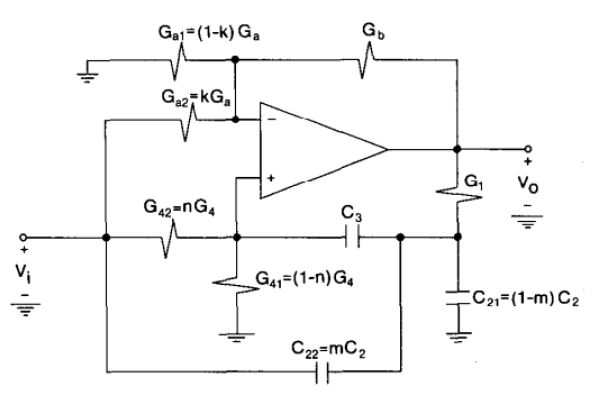
\includegraphics[width=0.5\textwidth]{Imagenes-Ej3/HPBSedra.PNG}
	\label{fig:HPBSedra}
	\caption{Circuito celda SGB-HPB}
\end{figure}
\subsubsection{Cálculo Analítico}
---
\subsubsection{Elecciones de diseño}
El análisis de sensibilidades que se obtiene del circuito, el cual coincide con lo publicado en el paper es la siguiente: 
\begin{center}
	\huge{\textcolor{red}{\textbf{Tabla sensibilidades}}}
\end{center}
En base a esta tabla se tomo especial cuidado en la elección de componentes y en el matcheo de impedancias.
Se tomaron como valor de los componentes...
Se eligió utilizar presets para las resistencias... Para ajustar el Q y el $\omega_0$ del filtro.
\subsubsection{Acoplamiento de Impedancias.}
Para que ambas etapas no se carguen entre si la impedancia de entrada de la segunda etapa debe ser mucho mayor a la de salida de la primera
\subsection{Respuesta en Frecuencia.}
Se realizó un análisis de Montecarlo a la respuesta en frecuencia del circuito, utilizando una tolerancia de las resistencias al 1$\%$ y capacitores al 10$\%$ obteniendo la siguiente disperción,
\subsubsection{Etapas.}
Se realizaron 2 etapas, ambas siendo el mismo tipo de celda, pero con distintos parámetros.
\subsubsection{Filtro definitivo.}
%
%\begin{figure}[H]
%	\centering
%	\includegraphics[width=0.4\textwidth]{/ImagenesEjercicio3/Graph.png}
%	\label{fig:graph}
%\end{figure}
\end{document}